%=====================================================================
%   LITERATURE REVIEW
%=====================================================================

\chapter{Literature review}
\label{ch:review}

\section{Biological Context}
\label{sec:biological-context}

Mycobacteria are a genus of bacteria with an unusually thick, waxy cell wall built around long-chain mycolic acids, which is the main reason they grow slowly and resist many standard antibiotics \citep{brennan_structure_2003}. The most clinically important species, \textit{Mycobacterium tuberculosis} (Mtb), is both slow-growing and pathogenic: it takes three to four weeks to form a colony and must be handled in a biosafety level 3 (BSL-3) facility \citep{sparks_mycobacterium_nodate}. Live single-cell imaging of Mtb is therefore very difficult, and \textit{Mycobacterium smegmatis} is used instead as a fast-growing, non-pathogenic model. It is not a perfect substitute, since Mtb divides differently at the single-cell level and doubles roughly every eighteen hours against three to five hours for \textit{M. smegmatis} \citep{chung_single-cell_2024,sparks_mycobacterium_nodate}. Slow-growing species need correspondingly long imaging runs to capture meaningful growth events, which is part of the motivation for an incubator that holds stable conditions over extended periods.

Bulk culture measurements average away important detail. Even within a clonal population, individual mycobacterial cells vary in growth rate, division timing and antibiotic susceptibility, partly because of their unusual unipolar growth pattern \citep{davis_defining_2016,aldridge_asymmetry_2012}. Cells also organise into larger structures: grown without detergent, mycobacteria align into bundles known as cords, a behaviour linked to virulence that also appears in nonpathogenic species \citep{julian_microscopic_2010}. Neither cell-to-cell variation nor cording survives a bulk measurement; both require live imaging at the single-cell and microcolony scale.

A common method for this is the agar-pad technique, where cells are sandwiched between a coverslip and a pad of agar and imaged from below on an inverted microscope \citep{joyce_modified_2011}. Agar pads support long imaging runs, but the sample chamber is open rather than sealed, so the bacteria are continuously exposed to whatever the surrounding environment does. Existing studies have focused on single cells or on fixed, mature colony structures, and little published work follows a microcolony live as it forms \citep{chung_single-cell_2024,aldridge_asymmetry_2012,davis_defining_2016,julian_microscopic_2010}. That is the gap this project addresses: a sealed, environmentally controlled stage-top system that holds imaging conditions over long continuous runs, making microcolony formation directly observable.

\section{Live-Cell Imaging Environmental Demands}
\label{sec:environmental-demands}

Live-cell microscopy places strict requirements on the sample environment. Cells must be held at a stable temperature, with controlled pH and minimal evaporation of the surrounding medium, or they mount stress responses that alter the processes being observed \citep{frigault_live-cell_2009}. In mammalian cell culture, pH is usually held with a bicarbonate buffer and a 5\% CO$_2$ atmosphere, alongside a relative humidity of 90 to 95\% to limit evaporation \citep{talebipour_facilitating_2024,coutu_probing_2013}. Standard cell incubators hold these conditions but are generally incompatible with microscopy, which has driven a shift toward compact stage-top systems that deliver heat, humidity and gas directly to the sample on the microscope itself \citep{talebipour_facilitating_2024}.

\subsection{Carbon dioxide requirements for mycobacteria}
\label{subsec:myco-co2-humidity}

Mycobacteria are not cultured the same way as mammalian cells. Both \textit{M. smegmatis} and \textit{M. tuberculosis} grow at around 37\textdegree{}C, but \textit{M. smegmatis} is non-fastidious. ATCC's handling instructions for the standard laboratory strain (mc\textsuperscript{2}155) list the required atmosphere simply as aerobic, with no added CO$_2$ \citep{atcc_mycobacterium_smegmatis}. \textit{M. tuberculosis} often needs 5 to 10\% CO$_2$, but mainly for primary isolation from clinical samples or when growing from very few cells: CO$_2$ substitutes for a biotin requirement in many clinical strains, a mechanism identified by \citet{schaefer_roles_1955} and still reflected in current culture media guidance \citep{hardy_diagnostics_middlebrook_2020}. Established laboratory strains grown to a reasonable density in liquid culture are commonly kept at 37\textdegree{}C in ordinary air, with a CO$_2$ incubator reserved for the mammalian host cells in infection experiments rather than for the bacteria \citep{nazarova_growing_2017}.

The incubator built here therefore does not need mammalian-style CO$_2$ control by default, and \textit{M. smegmatis} should grow well in ordinary air. The system should still support a controlled CO$_2$ atmosphere, but for a reason that should be stated precisely, because it is not the bacterium. This work is intended to progress toward host-cell infection models, in which mycobacteria are imaged interacting with mammalian tissue such as precision-cut lung slices. There it is the host tissue, not the bacterium, that fails without a bicarbonate-buffered 5\% CO$_2$ atmosphere \citep{nazarova_growing_2017,frigault_live-cell_2009}. Retaining a CO$_2$ loop is not over-engineering for \textit{M. smegmatis}; it is what allows the same chamber to be used later for infection imaging without a redesign.

\subsection{Temperature stability}
\label{subsec:temp-stability}

Temperature stability matters beyond simply keeping cells alive. \citet{grigorov_dynamic_2023} showed that shifting \textit{M. smegmatis} from 37\textdegree{}C down to 15\textdegree{}C halted cell division for around 24 hours and altered the expression of nearly a quarter of the genome within two hours, with growth-related genes downregulated and stress-response genes upregulated. A substantial deviation from the target temperature therefore does not just slow growth, it diverts the cell's resources toward survival, which risks interfering with the behaviour the incubator is meant to observe. It also suggests a useful incubator should support an adjustable setpoint rather than a single fixed temperature, since researchers may want to run temperature-shift experiments deliberately \citep{grigorov_dynamic_2023}. The mammalian host cells this platform is intended to serve next are no more demanding. They are cultured at 37\textdegree{}C \citep{frigault_live-cell_2009}, and it takes a downshift of a few degrees, to 32 to 35\textdegree{}C, to trigger a cold-shock response and slow their growth \citep{alfageeh_cold_2006}. Neither organism therefore needs holding to within a few tenths of a degree to stay healthy; a tighter band is a choice, made to match the systems reviewed and to limit the focal drift described in Section~\ref{subsec:drift-demands}.

Two approaches to holding temperature during imaging appear in the literature. Enclosing the whole microscope in a heated box is stable, but slow to settle and awkward to modify. Heating a small stage-top chamber around the sample is faster and more flexible, but more exposed to local disturbances: the objective lens touching the sample can act as a heat sink and cool it below setpoint right where it is being imaged \citep{frigault_live-cell_2009}, a small chamber is more sensitive to draughts or room temperature changes, and uneven heating can leave one part of the sample warmer than another.

\subsection{Evaporation and humidity}
\label{subsec:evaporation-humidity}

Small sample volumes are vulnerable to evaporation, which raises the osmolarity of the medium and stresses the cells \citep{frigault_live-cell_2009}. The standard fix is to humidify the air around the sample. Evidence from microscale cell assays points to a minimum relative humidity of about 95\%, since below that even small amounts of evaporation generate local currents strong enough to disturb the sample, an effect that worsens as chamber volume shrinks \citep{berthier_managing_2008,berthier_managing_2008-1}. A water reservoir inside the sealed chamber helps maintain this: it evaporates in place of the sample and buffers against small leaks in the seal \citep{berthier_managing_2008-1}.

\subsection{Focal-plane drift}
\label{subsec:drift-demands}

Focal-plane drift is a further constraint on long-duration imaging. Most drift comes from small temperature changes rather than mechanical movement, and even good laboratory air conditioning leaves a residual fluctuation of around 0.5\textdegree{}C \citep{adler_reducing_2003}. What matters is the rate of change rather than the absolute temperature, because different parts of a microscope have different thermal mass and settle at different rates. Left uncorrected, drift can exceed the resolution of the microscope, distort three-dimensional image stacks, and in time-lapse data become difficult to distinguish from real cell movement or growth \citep{adler_reducing_2003}.

Localised heat sources are themselves named as contributors to drift, including sample chamber heaters and objective heaters \citep{adler_reducing_2003}, the same components needed to hold the sample at a stable temperature. This is a direct design tension for a stage-top incubator: the heater that stabilises temperature at the sample can itself drive focal drift. Characterising drift in the finished system is therefore an important part of this project.

\section{Existing Stage-Top Incubator Systems}
\label{sec:existing-systems}

A number of commercial and open-source stage-top incubators already exist. The commercial systems (Ibidi, Okolab, Tokai Hit and LCI) are built to a high standard but are closed, proprietary and expensive. In principle none of them is specific to one organism: nothing about a heated chamber holding 37\,\textdegree{}C at a controlled humidity stops it hosting a bacterial sample. What they are is calibrated around mammalian cell culture, in their default setpoints, in the sample vessels they accept, and in the price point the mammalian cell-biology market will bear. The open-source and do-it-yourself (DIY) systems, built mostly by academic groups (Talebipour, Worcester, Ragazzini, Yan and ThermoCyte), reproduce the same core functions at a fraction of the cost, usually with an Arduino or similar microcontroller. This section works through each environmental variable in turn, rather than each system in turn, so that the commercial and DIY approaches to the same problem sit side by side. Two points are common to nearly all of these systems: bulkiness is a shared drawback, since a full chamber can be awkward to handle on a crowded stage, and some designs place heating elements directly next to the cell chamber, which risks interference with the experiment \citep{talebipour_facilitating_2024}; and a chamber does not need to be fully airtight to work well, since reducing leakage mainly lowers the CO$_2$ needed to hold a setpoint, and so the running cost, rather than being required for stability \citep{talebipour_facilitating_2024}.

\subsection{Temperature control}
\label{subsec:existing-temperature}

Three approaches to temperature control appear across the systems reviewed: continuous or proportional heating below saturation, used by Ibidi and Okolab; full closed-loop proportional-integral-derivative (PID) control, used by LCI and the DIY builds from Ragazzini, Yan and ThermoCyte; and simple bang-bang switching, used by Worcester's build \citep{noauthor_stage_nodate,okolab_stagetop_bl3,noauthor_incubator_2021,ragazzini_fabrication_2019,yan_establishment_2024,ocarroll_thermocyte_nodate,worcester_low-cost_2025}. PID gives the tightest holding, typically within a few tenths of a degree, at the cost of more complex electronics and tuning effort. Bang-bang is far simpler but accepts a wider, oscillating error band, and a heat-only PID design that cannot actively cool, as in Ragazzini's build, will always overshoot slightly above setpoint rather than settling on it.

How the heat is delivered also has optical consequences, which is easy to overlook when comparing systems on holding accuracy alone. \citet{ragazzini_fabrication_2019} heat their chamber through indium tin oxide (ITO) coated glass, but cut a hole in the ITO layer and fit a plain glass coverslip in its place, specifically to restore the transparency that phase-contrast imaging requires. Any heated window sits directly in the optical path, and reduced transmission through it has to be compensated by raising illumination intensity, which is the standard driver of phototoxicity and photobleaching in long time-lapse runs \citep{frigault_live-cell_2009}. Phototoxicity is not something the incubator controls, but the transparency of whatever material carries the heating element indirectly sets how hard the illumination has to work over a multi-day run.

Nearly every commercial system also heats the objective lens directly, whether as a built-in PID channel (LCI) or an add-on accessory (Tokai Hit, Ibidi). This is not a nice-to-have: Section~\ref{subsec:temp-stability} established that an unheated immersion objective acts as a heat sink and pulls the sample below setpoint at the exact point being imaged. Ibidi's chamber design, shown in Figure~\ref{fig:ibidi-diagram}, applies the same logic to the whole enclosure: the lid is held a few degrees above the plate, which creates a gradient that stops condensation forming on the optical path, while a separate humidity sensor and a pre-humidified gas mixture hold the chamber near saturation \citep{noauthor_stage_nodate}.

\begin{figure}[htbp]
    \centering
    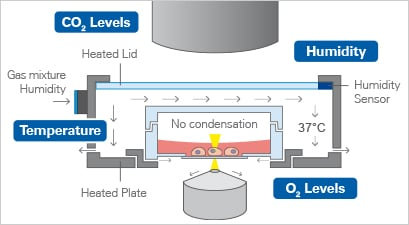
\includegraphics[width=0.44\linewidth]{figs/Lit Review/Ibidi.jpg}
    \caption[Ibidi temperature, humidity and gas control schematic]{\textbf{Ibidi stage-top incubator temperature, humidity and gas control schematic.} The heated lid is held above the heated plate to prevent condensation forming on the optical path, while a humidity sensor and pre-humidified gas mixture hold the chamber near saturation. Reproduced from \citet{noauthor_stage_nodate}.}
    \label{fig:ibidi-diagram}
\end{figure}

Given that \textit{M. smegmatis} tolerates a wider temperature range than the precision most of these systems target, the design question is not which method is most accurate in absolute terms, but which is simple enough to build on the STM32 platform already specified while still holding within whatever tolerance the biology needs. A basic PID loop is the more defensible default: Ragazzini and Yan both show it is achievable for well under EUR 300 in DIY components, it can be reused across all three environmental loops instead of mixing control schemes, and it holds a tighter band than the oscillating error of bang-bang switching.

\subsection{Carbon dioxide control}
\label{subsec:existing-co2}

Two ways of delivering CO$_2$ appear. The first is a pressurised cylinder feeding a solenoid valve under sensor feedback, used by Talebipour and Ragazzini and, commercially, as one of Tokai Hit's two cylinder options. The second is a larger premixed or in-line gas-mixing system, used by Yan's build and by LCI and Okolab \citep{talebipour_facilitating_2024,ragazzini_fabrication_2019,noauthor_tokai_nodate,yan_establishment_2024,noauthor_incubator_2021,okolab_stagetop_bl3}. Every system that controls CO$_2$ closes the loop with some form of non-dispersive infrared (NDIR) sensor and a valve, regardless of delivery route. ThermoCyte is the one system reviewed with no CO$_2$ control, since it is built for a flow-through setup where gas concentration is not the limiting variable \citep{ocarroll_thermocyte_nodate}. Unlike humidity, CO$_2$ is never left to hold its own level passively: it is continuously consumed and lost to leakage rather than settling toward an equilibrium.

The cylinder-and-solenoid route is the more defensible choice here. It is what the cheapest working DIY builds already use (Ragazzini sourced CO$_2$ from an aquarium supply rather than a laboratory gas line, correcting the setpoint from 5\% to 5.3\% to account for dilution by water vapour once the dry gas mixes with humidified chamber air), it needs no lab gas line, and it reuses the same sensor-and-valve logic as temperature control. The requirement here is narrower than matching the 5\% target every reviewed system is built around: the loop needs to exist, and to be accurate enough to be tuned up later, for the reason set out in Section~\ref{subsec:myco-co2-humidity}.

\subsection{Humidity control}
\label{subsec:existing-humidity}

There are two options for humidity control: an actively controlled external humidifier that blends humidified and dry gas before it reaches the chamber, used by Ibidi, Okolab, LCI and Tokai Hit's optional accessory; or a passive water reservoir inside the sealed, heated chamber that simply evaporates in place, used by Talebipour, Ragazzini and Yan \citep{noauthor_stage_nodate,okolab_stagetop_bl3,noauthor_incubator_2021,noauthor_tokai_nodate,talebipour_facilitating_2024,ragazzini_fabrication_2019,yan_establishment_2024}. The passive route seems ideal: it needs no extra sensor or control loop, and three of the five DIY systems rely on it successfully even while running PID on temperature and CO$_2$. It is also where the clearest practical failure shows up, though the problem is reservoir capacity and not the passive mechanism itself. Any small reservoir carried inside the system runs dry in hours to a few days: Worcester's holds 45 to 50\,mL and Tokai Hit's needs refilling every three to four days, neither of which fits a multi-day run.

The fix for capacity is moving the reservoir outside the chamber, with gas bubbling through it to pick up moisture on the way in. What Okolab's external module, Tokai Hit's optional humidifier and LCI's Incubator TW tank add on top of that is a sensor and closed loop holding relative humidity at a setpoint. A passive reservoir skips that loop and relies on whatever humidity the bubbling happens to produce at a given flow rate and reservoir size. Whether that is steady enough to hold over a multi-day run is not obvious and would need testing.

\subsection{Focal-plane drift}
\label{subsec:existing-drift}

None of the systems reviewed report a direct measurement of focal-plane drift. An unheated objective is a clear case: with no active control of its own, its temperature tracks the room rather than the sample, so an ambient swing pulls the objective and the actively stabilised stage apart at different rates, and that mismatch appears as drift. Heating the objective to the sample setpoint, as LCI, Tokai Hit and Ibidi all do, should reduce this driver.

The same fix can have the opposite effect, since objective heaters are also localised heat sources (Section~\ref{subsec:drift-demands}). A bang-bang or heat-only PID objective heater would place a small repeating temperature swing right next to the optics instead of removing one, where a tightly tuned PID loop would not. An objective heater is therefore neither simply good nor bad for drift; what matters is how well it is regulated. Since no reviewed system reports measuring the net effect, characterising drift in the finished incubator would be useful.

\subsection{Interface and monitoring}
\label{subsec:existing-interface}

All four commercial systems use a dedicated display or touchscreen, in some cases with remote or mobile monitoring; LCI's Android app and alarm function is the most complete example \citep{noauthor_incubator_2021,okolab_stagetop_bl3,noauthor_tokai_nodate}. Every DIY system reviewed uses a bare-bones host-computer or Arduino-LCD setup instead \citep{worcester_low-cost_2025,ragazzini_fabrication_2019,yan_establishment_2024,ocarroll_thermocyte_nodate}. Given the STM32 platform and host-side logging already specified, a simple serial link to a logging computer, the approach Worcester, Ragazzini and Yan all took, is sufficient for a lab prototype.

\subsection{Accuracy}
\label{subsec:existing-accuracy}

\citet{yan_establishment_2024} directly benchmarked their own system against three commercial systems on the same bench under the same protocol, alongside self-reported figures from other systems (Table~\ref{tab:accuracy_comparison}). Their own device, at $\pm$0.19\textdegree{}C and $\pm$0.13\% CO$_2$ by volume, sat within the same range as the commercial systems on temperature and comfortably within range on gas accuracy, despite being built at a fraction of the cost.

\begin{table}[htbp]
    \centering
    \caption[Reported control accuracy across incubator systems]{\textbf{Reported control accuracy across the incubator systems reviewed.} The first four rows come from a single bench test under one protocol \citep{yan_establishment_2024}; the remaining figures are self-reported by each system's own authors, under their own test conditions, and are not directly comparable.}
    \label{tab:accuracy_comparison}
    \small
    \setlength{\tabcolsep}{4pt}
    \renewcommand{\arraystretch}{1.15}
    \begin{tabular}{@{}>{\raggedright\arraybackslash}p{2.3cm}>{\raggedright\arraybackslash}p{2.0cm}>{\raggedright\arraybackslash}p{5.5cm}>{\raggedright\arraybackslash}p{3.0cm}@{}}
        \toprule
        \textbf{System} & \textbf{Type} & \textbf{Temperature} & \textbf{Gas (CO$_2$)} \\
        \midrule
        \multicolumn{4}{@{}l}{\textit{Benchmarked on one bench, one protocol} \citep{yan_establishment_2024}} \\
        Okolab & Commercial & 37.0$\pm$0.1/$\pm$0.3\textdegree{}C & $\pm$0.1\% vol \\
        Tokai Hit & Commercial & 37.0$\pm$0.3\textdegree{}C & $\pm$0.1\% vol \\
        Ibidi & Commercial & 37.0$\pm$0.2\textdegree{}C & $\pm$0.5\% vol \\
        Yan MIS & DIY & 37.0$\pm$0.19\textdegree{}C & $\pm$0.13\% vol \\
        \midrule
        \multicolumn{4}{@{}l}{\textit{Self-reported, from each system's own paper or website}} \\
        Ibidi & Commercial & 37.0 $\pm$ 0.2\textdegree{}C &  $\pm$ 0.2\% vol \\
        Talebipour & DIY & 37.0$\pm$0.1\textdegree{}C & --- \\
        Ragazzini & DIY & 37.0 $\pm$ 0.3\textdegree{}C  & --- \\
        ThermoCyte & DIY & 36.56$\pm$0.42\textdegree{}C  & --- \\
        Worcester & DIY & 36.8 $\pm$ 0.7\textdegree{}C & 5.3 $\pm$ 0.2\% vol  \\
        \bottomrule
    \end{tabular}
\end{table}

These figures should not all be weighted equally. Yan's numbers are the only ones measured on the same bench under the same protocol, which is what makes that comparison meaningful. Everything below the line is manufacturer- or author-reported under conditions that differ between studies and are rarely published in full, so those rows are best read as claims rather than measurements. Taken together, though, a carefully built DIY system using PID control reaches accuracy broadly comparable to commercial systems, even if the commercial systems remain more consistent overall.

A further limitation is that none of the systems reviewed report a continuous multi-day characterisation of the kind a mycobacterial microcolony experiment would demand. Whether these accuracies survive over 48 hours or longer, once reservoirs deplete, sensors drift and the lab's own day--night ambient cycle is superimposed on the chamber, is not established in this literature.

\subsection{Comparison and costs}
\label{subsec:existing-comparison}

Table~\ref{tab:incubator_comparison} collects the cost and control approach for temperature, CO$_2$ and humidity across every system covered. Three points follow from it.

First, PID is the practical standard wherever precision matters on temperature or CO$_2$: LCI, Ragazzini, ThermoCyte and Yan all use it. Bang-bang, as in Worcester's build, is simpler and cheaper but accepts a wider, oscillating error band. Humidity breaks this pattern, since Talebipour, Ragazzini and Yan all leave it to passive evaporation while actively controlling temperature and CO$_2$. Second, an objective heater is close to a standard feature across the commercial systems, for the heat-sink reason given in Section~\ref{subsec:temp-stability}, so one should be available whenever the incubator is used for imaging, either built in or as a separate laboratory accessory.

Third, and most directly relevant, none of these systems were developed with mycobacterial imaging in view. Nothing here rules these systems out for \textit{M. smegmatis}. A chamber that holds 37\,\textdegree{}C at controlled humidity will host it perfectly well. Worcester's build was validated against a commercial Ibidi system using mammalian doubling times, and nothing in that validation is specific to the cell type. The gap lies elsewhere. The commercial systems are priced for well-funded cell-biology laboratories and closed to modification, so a research group cannot add a sensor, change a setpoint range or adapt the chamber geometry. The DIY builds are cheap and modifiable but are individually documented one-off builds rather than characterised platforms. Across both categories the environmental envelope is set by mammalian defaults, which is more control than \textit{M. smegmatis} needs on CO$_2$, and says nothing about performance over the multi-day runs microcolony formation requires. A compact, modifiable incubator, scoped to what mycobacterial imaging actually demands and characterised over realistic run lengths, is the gap this project fills.

\begin{table}[htbp]
    \centering
    \caption[Comparison of stage-top incubator systems]{\textbf{Comparison of stage-top incubator systems reviewed.} Approximate cost (ZAR) and control approach. PID: closed-loop PID. Bang-bang: on/off switching. Active: sensor-driven or continuously driven, method not specified. Passive: no sensor-driven feedback. None: not controlled.}
    \label{tab:incubator_comparison}
    \small
    \setlength{\tabcolsep}{5pt}
    \renewcommand{\arraystretch}{1.15}
    \begin{tabular}{@{}>{\raggedright\arraybackslash}p{3.0cm}>{\raggedright\arraybackslash}p{2.6cm}>{\raggedright\arraybackslash}p{2.5cm}>{\raggedright\arraybackslash}p{2.9cm}>{\raggedright\arraybackslash}p{2.3cm}@{}}
        \toprule
        \textbf{System} & \textbf{Approx.\ cost} & \textbf{Temperature} & \textbf{CO$_2$} & \textbf{Humidity} \\
        \midrule
        \multicolumn{5}{@{}l}{\textit{Commercial (proprietary, not modifiable)}} \\
        Ibidi Silver Line & R\,423\,600 (full config.) & Active & Active (optional module) & Active \\
        Okolab BL3 & Not published & Active & Active & Active \\
        Tokai Hit & Not published & Active & Active & Passive \\
        LCI Incubator T & Not published & PID & PID & PID \\
        \midrule
        \multicolumn{5}{@{}l}{\textit{Open-source and DIY (modifiable)}} \\
        Talebipour mini-incubator & Not reported & Active & Active & Passive \\
        Worcester DIYncubator & R\,4\,060--4\,870 & Bang-bang & Bang-bang & Active \\
        Ragazzini incubator & R\,4\,870 & PID & PID & Passive \\
        Yan MIS & Not reported & PID & PID & Passive \\
        ThermoCyte & R\,3\,750  & PID & None & None \\
        \bottomrule
    \end{tabular}

    \vspace{3pt}
    \begin{minipage}{\textwidth}
        \footnotesize
        \textit{Notes:} Costs converted to ZAR at USD/ZAR~16.24 and EUR/ZAR~18.73 (September 2026). Ibidi's figure was confirmed against the current ibidi.com listing \citep{noauthor_stage_nodate} and Worcester's against \citet{worcester_low-cost_2025}. Ragazzini and ThermoCyte costs are as reported in \citet{ragazzini_fabrication_2019} and \citet{ocarroll_thermocyte_nodate}. For context, an undergraduate design report comparing commercial options found a World Precision Instruments chamber at R\,186\,700 and an Ibidi system at R\,227\,200 \citep{puccinelli_microscope_nodate}, broadly consistent with the Ibidi figure above; it is used here only for the market survey it documents, not as an independent technical result.
    \end{minipage}
\end{table}

\subsection{Microfluidic alternatives for bacterial imaging}
\label{subsec:microfluidic-alternatives}

Stage-top incubators are not the only route to long-duration bacterial imaging. A parallel line of work builds microfluidic culture devices that trap individual bacteria in defined channels and perfuse fresh medium past them, and at least one has been developed specifically for \textit{M. smegmatis} \citep{wang2021development,golchin_microfluidic_2012}. These do not close the same gap, for two reasons. They do not replace an incubator but sit inside one, so the control problem this project addresses remains unsolved by that route. And they confine cells to chambers roughly 0.9\,\textmu m in height precisely to force growth into a single two-dimensional layer, which engineers away the multicellular organisation, cording and microcolony architecture that this project sets out to observe \citep{wang2021development}. Microfluidic platforms and stage-top incubators therefore answer different questions rather than competing.

\section{Multivariable Control of Coupled Environmental Loops}
\label{sec:multivariable-control}

Section~\ref{sec:existing-systems} surveyed how existing incubators generate and sense temperature, CO$_2$ and humidity, largely as three separate problems. What it did not address is what happens when all three are actuated at once in the same enclosure, which is the control problem this project actually has to solve. A wider literature on coupled temperature, humidity and CO$_2$ control, drawn from bioprinting, industrial climate testing and greenhouse engineering, gives a clearer picture of how difficult that coupling is and how it is normally handled.

\subsection{Why temperature, humidity and CO$_2$ are coupled}
\label{subsec:why-coupled}

\citet{matamoros_temperature_2020} built a decoupled PID controller for a bioprinter atmospheric enclosure and, citing \citet{yinping_expert_2017} among others, note that temperature and humidity are ``highly related variables, so their simultaneous control is complex and requires fine tuning.'' The coupling is not a minor effect: relative humidity was found to drop by 2 to 3\% for every 1\textdegree{}C rise in temperature, and without an active controller both variables fluctuated over a wide range together rather than settling independently. CO$_2$ adds a further layer of cross-coupling, and Matamoros et al. found it significant enough that they excluded CO$_2$ from their PID loop entirely, injecting it open-loop through a solenoid valve rather than closing a third feedback loop around it \citep{matamoros_temperature_2020}.

This is a direct warning for a project where temperature, humidity and CO$_2$ are all meant to be actively held in a small sealed chamber: actuating one variable will disturb the others, and the difficulty of that interaction should not be underestimated on the basis of the single-loop PID descriptions in Section~\ref{sec:existing-systems}, none of which report having characterised cross-coupling directly.

\subsection{Modelling coupled enclosures}
\label{subsec:modelling-enclosures}

A recurring approach is to model the enclosure as a lumped heat balance and a lumped water-vapour mass balance, both non-linear ``in minus out'' differential equations of the general form used throughout temperature and humidity control processes \citep{buonomano_temperature_2017,kapen_energy_2019}. \citet{matamoros_temperature_2020} write the vapour balance for their enclosure as

\begin{equation}
\rho V \frac{d(d_n)}{dt} = G_a \rho d_c + D_n - G_a \rho d_n
\label{eq:water-balance}
\end{equation}

where $d_n$ is the enclosure's inner humidity, $d_c$ that of the air supplied to it, $G_a$ the air mass flow rate, $D_n$ the moisture added by the actuator and $\rho$ the density of air, with a matching heat balance in the same form. Applying the Laplace transform gives first-order transfer functions for temperature and humidity, which is the standard route from a physical balance equation to a form a PID controller can be designed around \citep{matamoros_temperature_2020}. \citet{riahi_intelligent_2020} apply the same balance-equation structure to a much larger and leakier enclosure, an agricultural greenhouse, and validate the resulting model against several days of real sensor data rather than simulation alone; that the same approach holds across enclosures this different in scale is a reasonable indication it would generalise down to the much smaller chamber here.

Two practical details are worth carrying forward. \citet{matamoros_temperature_2020} found their experimental and theoretical transfer functions diverged slightly until an exponential dead-time term was added, attributed to sensor response lag rather than the physical system, so any sensor used here should be characterised for that lag before poor control performance is blamed on the plant. And both transfer functions were fitted and validated against real test data using MATLAB's System Identification Toolbox, with an initial Ziegler--Nichols tuning then hand-corrected to remove overshoot: a practical route to a working controller that does not require every physical constant to be known in advance.

\subsection{Coupled versus decoupled control architectures}
\label{subsec:coupled-decoupled}

There is no settled answer in this literature to whether temperature and humidity should be controlled by one coupled controller or by two independent loops. \citet{matamoros_temperature_2020} note that some prior work proposes coupled controllers while other work, including their own, proposes decoupled ones, and choose the decoupled route deliberately to keep the PID design and tuning tractable. \citet{riahi_intelligent_2020} make the same architectural choice for a fuzzy rather than PID controller, separating temperature error and humidity error into two independent loops; the decision to decouple holds across both algorithm types even though the control law differs. For a project with three coupled loops on a single embedded platform, that is a reasonable argument for the same decoupled pattern already found throughout Section~\ref{sec:existing-systems}. A coupled controller may give tighter performance, but it adds design and tuning complexity that this literature treats as one of two competing approaches rather than a settled requirement.

\subsection{Beyond PID}
\label{subsec:beyond-pid}

PID is not the only option for holding a coupled multivariable system at setpoint. \citet{chen_review_2025}, reviewing environmental control for agricultural greenhouses, place PID at the start of a progression that also includes fuzzy, feedback, adaptive, model-predictive and neural-network control, and conclude that PID remains ``the simplest and most widely used method'' but is ``no longer sufficient'' as control demands grow. For this project that sophistication is not obviously worth adopting. PID is the only one of those algorithms used anywhere in Section~\ref{sec:existing-systems}, and the only one with a demonstrated low-cost single-microcontroller implementation in the incubator literature. The disadvantages of the alternatives, principally high model dependency for model-predictive control and high data and training demand for neural networks, are a poor match for a system with a single prototype to tune on and no operating history to learn from. PID, run as decoupled per-variable loops, remains the stronger choice; the more advanced algorithms are worth revisiting only if PID's coupling-driven error proves too large once the finished system is characterised.

\section{Summary of the Literature}
\label{sec:review-summary}

The literature reviewed leaves a specific and unfilled space. The biology sets the requirement: \textit{M. smegmatis} needs a stable, adjustable temperature and protection from evaporation over runs long enough for a microcolony to form, but not the 5\% CO$_2$ atmosphere mammalian culture is built around, although a CO$_2$ channel must remain available for the host-cell infection models this platform is intended to serve next (Section~\ref{subsec:myco-co2-humidity}). The microfluidic devices that come closest by organism do not address environmental control at all, and deliberately suppress the multicellular growth this project exists to observe. The control literature establishes that the three variables are genuinely cross-coupled and that decoupled per-variable PID is the sound starting architecture, yet no incubator in Section~\ref{sec:existing-systems} reports characterising that coupling in a chamber of this size.

No single system, therefore, combines compact and modifiable hardware, an environment scoped to mycobacterial imaging while retaining CO$_2$ capability, decoupled multi-loop control on one embedded platform, and characterised long-duration performance. That combination is what this project sets out to build and demonstrate.